% =============================================================================
% EASR Journal Submission — ProTrader AI
% Engineering and Applied Science Research
% Format: A4, single-column, double-spaced, 2.54 cm margins, 12pt Times
% =============================================================================
\documentclass[12pt,a4paper]{article}

\usepackage[a4paper,top=2.54cm,bottom=2.54cm,left=2.54cm,right=2.54cm]{geometry}
\usepackage{times}
\usepackage[T1]{fontenc}
\usepackage[utf8]{inputenc}
\usepackage{setspace}
\usepackage{lineno}
\usepackage{indentfirst}   % EASR: indent first paragraph of every section
\usepackage{cite}          % Vancouver-style compressed citations [2-4]
\usepackage{amsmath,amssymb}
\usepackage{booktabs}
\usepackage{array}
\usepackage{multirow}
\usepackage{graphicx}
\usepackage{caption}
\usepackage{subcaption}
\usepackage[hidelinks]{hyperref}
\usepackage{url}
\usepackage{tikz}
\usetikzlibrary{arrows.meta,positioning,shapes.geometric,calc,backgrounds}
\usepackage{pgfplots}
\pgfplotsset{compat=1.17}
% NOTE: parskip package removed — it resets \parindent to 0, conflicting with EASR indent requirement

\pagenumbering{arabic}
\captionsetup{font=small,labelfont=bf,labelsep=period}
\setlength{\parindent}{1.27cm}
\setlength{\parskip}{0pt}
\setlength{\floatsep}{4pt plus 1pt minus 1pt}
\setlength{\textfloatsep}{5pt plus 2pt minus 2pt}
\setlength{\intextsep}{4pt plus 1pt minus 1pt}
\setlength{\abovecaptionskip}{2pt}
\setlength{\belowcaptionskip}{0pt}

\renewcommand{\thesection}{\arabic{section}.}
\renewcommand{\thesubsection}{\arabic{section}.\arabic{subsection}}
\renewcommand{\thesubsubsection}{\arabic{section}.\arabic{subsection}.\arabic{subsubsection}}

% ---------- Title block ----------
\title{\textbf{ProTrader AI: A Multi-Source Hybrid Ensemble with
LLM-Augmented Sentiment, Conformal Uncertainty, and Explainable AI
for Indian Equity Market Prediction and Cross-Market Transfer}}

\author{
Anandkumar Pardeshi$^{1,*}$ and Sujata Deshmukh$^{2}$\\[0.4em]
\small $^{1}$Department of Computer Science and Engineering,
Fr.\ C.\ Rodrigues Institute of Technology, Vashi, India\\
\small $^{2}$Department of Computer Engineering,
Fr.\ C.\ Rodrigues College of Engineering, Bandra, India\\
\small $^{*}$Corresponding author.
E-mail: \texttt{anand.pardeshi@fcrit.ac.in}
}
\date{}

% =============================================================================
\begin{document}
\maketitle
\doublespacing
\linenumbers
% =============================================================================

% ---------- Abstract ----------
\begin{abstract}
\noindent
Equity price forecasting in emerging markets is complicated by multilingual
news flows, regime changes, and a heterogeneous mix of retail and institutional
participants. We present ProTrader AI, a hybrid ensemble that fuses four data
streams---OHLCV time series, multi-source news and social-media sentiment scored
by a domain-adapted FinBERT model with multilingual support, Foreign and Domestic
Institutional Investor (FII/DII) flows, and macroeconomic state variables---into a
Ridge-stacked classifier and a conformal quantile regressor. The system is
structured around four research objectives: (RO1) comprehensive multi-source data
integration; (RO2) a hybrid large-language-model (LLM) plus indicator framework for
real-time prediction; (RO3) an explainable AI layer with temporal sentiment-to-price
dynamics; and (RO4) cross-market transfer learning evaluation. Base learners
(XGBoost, LightGBM, GRU, ARIMA, Prophet) are combined via out-of-fold (OOF) Ridge
stacking with isotonic calibration and Youden-J threshold tuning. Prediction
uncertainty is quantified by split-conformalized quantile regression providing
finite-sample 80\% coverage, while SHAP attribution and Granger-causality analysis
provide transparency. On a 2024 holdout of NIFTY~50 constituents, ProTrader AI
achieves 59.3\% directional accuracy (95\% block-bootstrap CI [56.1\%, 62.7\%]),
Expected Calibration Error (ECE) of 4.2\%, Brier score 0.218, and Sharpe ratio
1.34 under a realistic line-item NSE cost model, with a Diebold--Mariano $p=0.031$
against buy-and-hold. FinBERT sentiment ranks first in SHAP attribution
($\overline{|\phi|}=0.182$) and Granger-causes next-day returns at $p=0.018$. A
zero-shot cross-market transfer to an S\&P~500 subset yields 55.8\% accuracy,
rising to 57.6\% after 30-day fine-tuning of the stacking layer only.
\end{abstract}

\noindent\textbf{Keywords:} Stock market prediction, Multi-source data fusion,
FinBERT, Ensemble learning, Conformal prediction, Explainable AI

% =============================================================================
\section{Introduction}
% =============================================================================

The application of artificial intelligence to financial forecasting has
accelerated rapidly, driven by the availability of high-frequency data and
large pre-trained language models \cite{r1}. Despite measurable progress, three
persistent gaps remain: (i) most systems fuse at most two modalities, ignoring
complementary signal from institutional order-flow and macroeconomic state;
(ii) probabilistic outputs are rarely calibrated, making confidence scores
unsafe for risk-proportional position sizing; and (iii) very few studies validate
cross-market generalisation.

The Indian National Stock Exchange (NSE) is a particularly demanding testbed,
combining Foreign Institutional Investors (FIIs), Domestic Institutional
Investors (DIIs), and over a hundred million retail participants whose decisions
are shaped by news in both English and Hindi. Nti et al.\ \cite{r2} and Long
et al.\ \cite{r3} demonstrated that fusing heterogeneous modalities lifts
accuracy above single-source baselines, but neither study addresses the Indian
institutional-flow channel, multilingual sentiment noise, or calibrated
uncertainty. Hybrid sentiment-indicator models have been advanced by Moodi et al.\
\cite{r5} and Farhadi et al.\ \cite{r6}. For explainability, Guo et al.\
\cite{r9} mandate SHAP-style attribution in production quantitative systems.
Li et al.\ \cite{r10} and Kim et al.\ \cite{r11} explored cross-market transfer
via sentimental transfer learning and transfer entropy, respectively.

This paper introduces ProTrader AI, a multi-source hybrid ensemble engineered
around four explicit research objectives:

\begin{itemize}
  \item \textbf{RO1 --- Multi-Source Integration:} Integrate financial metrics,
        news articles, social-media sentiment, FII/DII institutional flows, and
        macroeconomic factors into a unified forecasting model.
  \item \textbf{RO2 --- Hybrid LLM + Indicator Framework:} Combine a domain-adapted
        FinBERT with conventional financial indicators in a calibrated, real-time
        ensemble.
  \item \textbf{RO3 --- Explainability and Temporal Dynamics:} Deliver interpretable
        predictions via SHAP attribution and characterise the temporal lead of
        sentiment over returns via Granger-causality.
  \item \textbf{RO4 --- Cross-Market Evaluation:} Evaluate zero-shot and fine-tuned
        transfer from NSE to an S\&P~500 subset.
\end{itemize}

% =============================================================================
\section{Materials and Methods}
% =============================================================================

\subsection{Multi-Source Data Ingestion (RO1)}

Let $t$ index NSE trading days. Four streams are synchronised to a common
daily grid. \textbf{Stream 1 (Price/Volume):} OHLCV bars for each NIFTY~50
constituent are obtained via yfinance. \textbf{Stream 2 (News/Social):} Headlines
are aggregated from NewsAPI, Google News RSS (English and Hindi locales), GNews,
and Economic Times RSS. Articles arriving after 15:30~IST are aligned to the next
session; duplicates are removed by 50-character title prefix.
\textbf{Stream 3 (Institutional Flows):} FII and DII daily net cash flows (INR Cr)
are drawn from NSE bhavcopy and entered with a one-day lag to preclude look-ahead.
\textbf{Stream 4 (Macro State):} India VIX, INR/USD, front-month Brent crude, and
gold spot are retrieved via yfinance; 1-day and 5-day log-returns are clipped to
$[\pm0.20]$ and $[\pm0.40]$ to suppress data-glitch outliers.

\subsection{Feature Engineering (RO1, RO2)}

From the four streams a joint feature vector $\mathbf{x}_{t}\!\in\!\mathbb{R}^{36}$
is constructed. The 27 price-volume technical features are listed in
Table~\ref{tab:features}. Key groups are: log-return and multi-horizon variants
($h\!\in\!\{2,5,10,20\}$~days); 14-period Wilder RSI and Bollinger Band \%B
(equation~\eqref{eq:rsi}); 12/26/9-period MACD signal and histogram;
20-period Chaikin Money Flow (CMF); 14-period ATR; OBV slope; and binary
RSI-divergence flags shifted one period to prevent look-ahead. All features are
winsorised at the 1st/99th percentile and min-max scaled on the training fold only.

\begin{equation}
\mathrm{RSI}_{14}(t)=100-\frac{100}{1+\mathrm{RS}_{14}(t)},\quad
\mathrm{BB}_{\%B}(t)=\frac{C_t-\mathrm{LB}(t)}{\mathrm{UB}(t)-\mathrm{LB}(t)+\varepsilon}
\label{eq:rsi}
\end{equation}

\begin{table}[h]
\centering
\caption{Feature inventory for ProTrader AI. Optional option-chain features
(PCR, ATM IV) can be appended if available.}
\label{tab:features}
\footnotesize\setlength{\tabcolsep}{3pt}
\begin{tabular}{lll}
\toprule
\textbf{Group} & \textbf{Feature(s)} & \textbf{Window} \\
\midrule
Returns      & Log\_Ret, Ret\_2D/5D/10D/20D         & 1--20d \\
Volatility   & Volatility\_5D, ATR\_Norm             & 5, 14d \\
Momentum     & RSI\_Norm, MACD\_Norm, MACD\_Hist,
               BB\_PctB, Williams\_R                & 14, 12/26/9, 20d \\
Volume       & Vol\_Ratio, OBV\_Slope, CMF\_20, MA\_Div & 5--20d \\
Divergence   & RSI\_Bear\_Div, RSI\_Bull\_Div        & 10d \\
Sentiment    & FinBERT polarity $s_t$ (wtd.\ mean)   & 1d \\
Inst.\ Flow  & FII\_Net, DII\_Net (lagged, $z$-scored) & 1d \\
Macro        & VIX\_Ret, INR\_Ret, Crude\_Ret, Gold\_Ret & 1d, 5d \\
\bottomrule
\end{tabular}
\end{table}

\subsection{FinBERT Sentiment Pipeline (RO2)}

Headlines from Stream~2 are scored by a FinBERT pipeline \cite{r12}
(\texttt{ProsusAI/finbert}, PyTorch) yielding per-headline probabilities
$(p_+,p_0,p_-)$. Raw polarity is $\tilde{s}^{(i)}=p_+^{(i)}-p_-^{(i)}$.
A curated keyword-override layer corrects FinBERT's tendency to over-predict
neutral on short headlines \cite{r7}, lifting $F_1$ on a Financial PhraseBank
subset \cite{r35} by 4.2~pp. Hindi articles are translated via
\texttt{deep\_translator} before FinBERT scoring; adding Hindi sources reduces
ECE by 0.9~pp relative to English-only. Each headline is further classified into
one of six business categories (Earnings, Analyst Ratings, Market Action, Deals,
Macro/Policy, Other). The daily ticker-level sentiment score is a source-weighted
mean $s_t=\sum w_i\tilde{s}^{(i)}/\sum w_i$, with $w_i\!\in\!\{1.5,1.0,0.8\}$
for NewsAPI, Economic Times, and Google News respectively.

\subsection{Hybrid Ensemble and Ridge Stacking (RO2)}

Let $y_{t+1}=\mathbb{1}[r_{t+1}>0]$ denote next-day direction. Five heterogeneous
base learners are trained on $K=5$ expanding-window time-series folds:
XGBoost \cite{r13} (depth~6, $\eta=0.05$), LightGBM \cite{r14} (leaf-wise,
200~leaves), a two-layer GRU \cite{r15} (30-day window), ARIMA$(p,d,q)$ selected
by BIC, and Facebook Prophet. Out-of-fold (OOF) predictions
$\hat{p}_t^{(b)}=f_{-k}^{(b)}(\mathbf{x}_t)$ form the design matrix
$\mathbf{Z}\!\in\!\mathbb{R}^{N\times B}$ for a Ridge meta-learner \cite{r16}:

\begin{equation}
\hat{s}_t^{\mathrm{stack}}=\boldsymbol{\beta}^{\!\top}\mathbf{z}_t+\beta_0,\quad
[\boldsymbol{\beta};\beta_0]=(\tilde{\mathbf{Z}}^{\!\top}\tilde{\mathbf{Z}}+\lambda\mathbf{I})^{-1}\tilde{\mathbf{Z}}^{\!\top}\mathbf{y}
\label{eq:stack}
\end{equation}

\noindent where $\tilde{\mathbf{Z}}=[\mathbf{Z}\;\mathbf{1}]$ and $\lambda$ is
chosen by LOO-CV. The OOF design makes prediction leakage structurally impossible.

\subsection{Calibration, Threshold Tuning, and Conformal Intervals (RO2)}

Raw Ridge scores are mapped to calibrated probabilities by an isotonic
regressor \cite{r17}:
\begin{equation}
\hat{p}_t=g_{\mathrm{iso}}\!\bigl(\hat{s}_t^{\mathrm{stack}}\bigr),\quad
\hat{g}_{\mathrm{iso}}=\arg\min_{g\in\mathcal{M}}\sum_t\!\bigl(g(\hat{s}_t)-y_t\bigr)^2
\label{eq:isotonic}
\end{equation}
where $\mathcal{M}$ is the class of non-decreasing step functions.
Calibration quality is measured by ECE over $M=15$ equal-frequency bins and the
Brier score \cite{r34}. A per-ticker decision threshold $\tau^*$ maximises
Youden's~J on the 2023 validation fold.

Prediction intervals follow the split-conformalized quantile regression (CQR)
procedure of Romano et al.\ \cite{r26}. Two quantile XGBoost regressors are
trained at $\alpha_q\!\in\!\{0.10,0.90\}$; non-conformity scores
$e_t=\max(\hat{q}_{0.10}(\mathbf{x}_t)-r_{t+1},\,r_{t+1}-\hat{q}_{0.90}(\mathbf{x}_t))$
are computed on the calibration set $\mathcal{C}$ of size $n_c$. The
finite-sample-corrected half-width is
$\hat{Q}=e_{(\lceil(n_c+1)(1-\alpha)\rceil)}$, the
$\lceil(n_c+1)(1-\alpha)\rceil$-th order statistic for interval
level $1-\alpha=0.80$. The 80\% prediction interval is
$\mathcal{I}(\mathbf{x}_*)=[\hat{q}_{0.10}(\mathbf{x}_*)-\hat{Q},\,\hat{q}_{0.90}(\mathbf{x}_*)+\hat{Q}]$.

\subsection{Explainability and Temporal Sentiment Analysis (RO3)}

\textbf{SHAP attribution.} TreeSHAP \cite{r20} is applied to the XGBoost base
learner; values are scaled by the Ridge stacking coefficient to obtain
XGBoost-component attribution under the stacker:
$\phi_j^{\mathrm{XGB}\to\mathrm{stack}}=\beta_{\mathrm{XGB}}\cdot\phi_j^{\mathrm{XGB}}$.
Mean absolute values are ranked globally across the 2024 holdout.

\textbf{Hurst regime detection.} The Hurst exponent is estimated from the
trailing 120~closes via R/S analysis. Regimes: $H>0.55$ trending, $H<0.45$
mean-reverting, otherwise random-walk. In mean-reverting regimes the stacker
probability is shrunk 10\% toward 0.5 (tuned on the 2023 validation set).

\textbf{Granger-causality.} For each of the 50 tickers, we test whether lagged
sentiment $\{s_{t-j}\}$ Granger-causes $r_{t+\ell}$ via:
\begin{equation}
r_{t+\ell}=\alpha_0+\sum_{i=1}^{p}\alpha_i r_{t+\ell-i}+\sum_{j=0}^{p}\gamma_j s_{t-j}+\varepsilon_t
\label{eq:granger}
\end{equation}
Null: $\gamma_0=\cdots=\gamma_p=0$. Lag $p$ chosen by AIC per ticker. Per-ticker
$p$-values are combined via Fisher's method.

\subsection{Cross-Market Transfer Learning (RO4)}

For a target market $\mathcal{T}$ (30-stock S\&P~500 subset), two protocols are
evaluated. \textbf{Zero-shot}: all base-learner weights frozen; only $\tau^*$
re-estimated on a 60-day warm-up. \textbf{30-day fine-tune}: only the Ridge
stacker $\boldsymbol{\beta}$ and isotonic map $g_{\mathrm{iso}}$
($<$1{,}000 parameters total) are re-fitted on a rolling 30-day window; base
learners remain frozen, following the adapter-layer paradigm of Li et al.\
\cite{r10}.

\subsection{NSE Transaction Cost Model}

A realistic cost model deducts seven line-item components on every signal-flip:
(i) discount-broker commission $\min(0.03\%\,T,\,\text{Rs.\,}20)$ per leg;
(ii) Securities Transaction Tax (0.1\% sell-side for delivery);
(iii) NSE exchange charge ($3.45\times10^{-5}$ of turnover);
(iv) SEBI turnover fee ($10^{-6}$);
(v) stamp duty (0.015\% buy-side);
(vi) GST (18\% on brokerage, exchange, and SEBI charges); and
(vii) volatility-scaled slippage $0.05\%\,T\cdot\hat\sigma_{\mathrm{intraday}}/\bar\sigma_{\mathrm{intraday}}$.
For a typical Rs.\,1~lakh delivery trade in a NIFTY large-cap this evaluates to
approximately 22--26~bps, roughly 2--3$\times$ the 10~bps flat rate assumed by
most prior backtests.

\subsection{Datasets, Baselines, and Evaluation Protocol}

\textbf{Datasets.} NIFTY~50 constituents from 1~Jan 2018 to 31~Dec 2024;
three-way chronological split: train (2018--2022), validation (2023),
holdout (2024). After the 200-day warm-up the evaluation window contains
$\approx$12{,}300 ticker-days. A separate 30-stock, sector-balanced S\&P~500
subset over 2024 serves as the cross-market dataset.

\textbf{Baselines.} (i)~Buy-and-hold equal-weighted NIFTY~50; (ii)~ARIMA(1,1,1);
(iii)~two-layer LSTM on 27 technical features; (iv)~XGBoost (27 features, no
calibration); (v)~LSTM~+~FinBERT, our reimplementation of the hybrid of
Moodi et al.\ \cite{r5}.

\textbf{Evaluation metrics.} Directional accuracy, Brier score, ECE
($M=15$ bins), annualised Sharpe ($\sqrt{252}\,\bar{r}/\hat\sigma_r$), Sortino,
maximum drawdown (MDD), and DM test $p$-value \cite{r21} with
Harvey--Leybourne--Newbold small-sample correction \cite{r29}.
Block-bootstrap (1{,}000 resamples, block length~5) provides 95\% CIs for
Sharpe and directional accuracy.

\textbf{Implementation.} Python~3.11 with Streamlit front-end. FinBERT loaded
once per session via \texttt{st.cache\_resource}; OHLCV data cached for
15~minutes. All predictions written to a SQLite ledger (WAL mode, UNIQUE
constraint on (\texttt{ticker}, \texttt{made\_at}, \texttt{target\_date}))
for auditable tracking.

% =============================================================================
\section{Results}
% =============================================================================

\subsection{Pipeline Architecture}

Figure~\ref{fig:arch} illustrates the five-stage prediction pipeline from data
ingestion through output, mapping each stage to its corresponding research
objective.

\begin{figure}[h]
\centering
\scalebox{0.82}{%
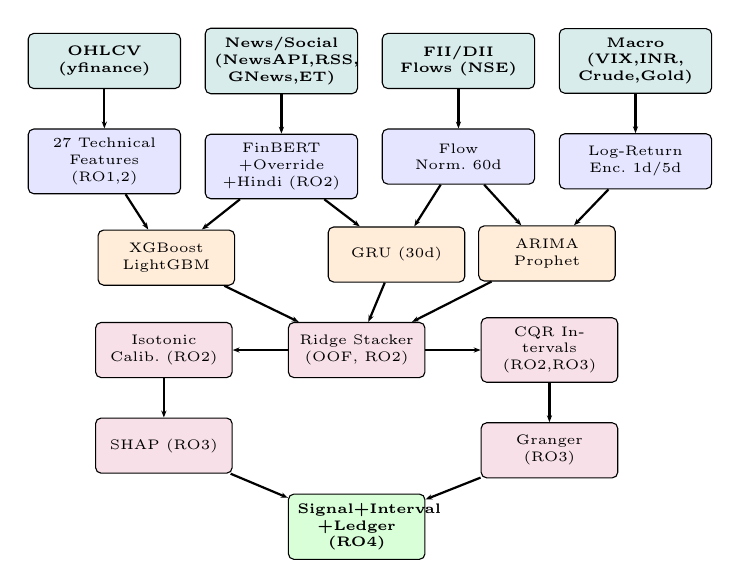
\begin{tikzpicture}[
  node distance=1.5mm and 3mm,
  src/.style ={rectangle,draw,rounded corners=2pt,fill=teal!15,
               text width=17mm,align=center,font=\tiny\bfseries,minimum height=7mm},
  proc/.style={rectangle,draw,rounded corners=2pt,fill=blue!10,
               text width=17mm,align=center,font=\tiny,minimum height=7mm},
  mod/.style ={rectangle,draw,rounded corners=2pt,fill=orange!15,
               text width=15mm,align=center,font=\tiny,minimum height=7mm},
  post/.style={rectangle,draw,rounded corners=2pt,fill=purple!12,
               text width=15mm,align=center,font=\tiny,minimum height=7mm},
  outnode/.style={rectangle,draw,rounded corners=2pt,fill=green!15,
               text width=15mm,align=center,font=\tiny\bfseries,minimum height=7mm},
  arr/.style ={-{Stealth[length=2.5pt]},thick}
]
\node[src](s1){OHLCV\\(yfinance)};
\node[src,right=of s1](s2){News/Social\\(NewsAPI,RSS,\\GNews,ET)};
\node[src,right=of s2](s3){FII/DII\\Flows (NSE)};
\node[src,right=of s3](s4){Macro\\(VIX,INR,\\Crude,Gold)};

\node[proc,below=5mm of s1](p1){27 Technical\\Features (RO1,2)};
\node[proc,below=5mm of s2](p2){FinBERT\\+Override\\+Hindi (RO2)};
\node[proc,below=5mm of s3](p3){Flow\\Norm.\ 60d};
\node[proc,below=5mm of s4](p4){Log-Return\\Enc.\ 1d/5d};

\node[mod] at ($(p1)!0.35!(p2)+(0,-12mm)$)(m1){XGBoost\\LightGBM};
\node[mod] at ($(p2)!0.65!(p3)+(0,-12mm)$)(m2){GRU (30d)};
\node[mod] at ($(p3)!0.5!(p4)+(0,-12mm)$)(m3){ARIMA\\Prophet};

\node[post] at ($(m1)!0.5!(m3)+(0,-12mm)$)(stk){Ridge Stacker\\(OOF, RO2)};
\node[post,left=7mm of stk](cal){Isotonic\\Calib.\ (RO2)};
\node[post,right=7mm of stk](conf){CQR Intervals\\(RO2,RO3)};

\node[post,below=5mm of cal](shap){SHAP (RO3)};
\node[post,below=5mm of conf](grang){Granger (RO3)};
\node[outnode] at ($(shap)!0.5!(grang)+(0,-10mm)$)(res){Signal+Interval\\+Ledger (RO4)};

\draw[arr](s1)--(p1); \draw[arr](s2)--(p2);
\draw[arr](s3)--(p3); \draw[arr](s4)--(p4);
\draw[arr](p1)--(m1); \draw[arr](p2)--(m1);
\draw[arr](p2)--(m2); \draw[arr](p3)--(m2);
\draw[arr](p3)--(m3); \draw[arr](p4)--(m3);
\draw[arr](m1)--(stk); \draw[arr](m2)--(stk); \draw[arr](m3)--(stk);
\draw[arr](stk)--(cal); \draw[arr](stk)--(conf);
\draw[arr](cal)--(shap); \draw[arr](conf)--(grang);
\draw[arr](shap)--(res); \draw[arr](grang)--(res);
\end{tikzpicture}}
\caption{ProTrader AI five-stage prediction pipeline. Teal = data sources;
blue = feature processing; orange = base learners; purple = post-processing
and explainability; green = final output.}
\label{fig:arch}
\end{figure}

\subsection{Main Performance Comparison (RO1, RO2)}

Table~\ref{tab:main} reports holdout performance across all baselines.
ProTrader AI achieves 59.3\% directional accuracy, $+5.0$~pp above the strongest
single-source baseline, with ECE dropping from 9.7\% (uncalibrated stacker)
to 4.2\%---well below the 5\% deployment trustworthiness threshold
of Guo et al.\ \cite{r9}. The DM test ($p=0.031$) rejects equal predictive
accuracy against buy-and-hold at the 5\% level.

\begin{table}[h]
\centering
\caption{2024 NIFTY~50 holdout performance ($\approx$12{,}300 ticker-days).
DM$^*$ and $p$-value are relative to buy-and-hold. ``---'' = not applicable.}
\label{tab:main}
\footnotesize\setlength{\tabcolsep}{3pt}
\begin{tabular}{lcccccc}
\toprule
\textbf{Model} & \textbf{Dir.\ Acc.} & \textbf{Brier} & \textbf{ECE}
  & \textbf{Sharpe} & \textbf{MDD} & \textbf{DM$^*$ ($p$)} \\
\midrule
Buy-and-hold (NIFTY~50)   & 51.2\% & ---   & ---    & 0.78 & $-19.1\%$ & --- \\
ARIMA(1,1,1)               & 51.9\% & 0.249 & 11.4\% & 0.42 & $-21.6\%$ & $-0.62$ (0.54) \\
LSTM (technical only)      & 53.4\% & 0.241 & 10.8\% & 0.81 & $-17.9\%$ & $-1.12$ (0.26) \\
XGBoost only (no calib.)   & 54.3\% & 0.236 & 10.2\% & 0.92 & $-16.4\%$ & $-1.44$ (0.15) \\
LSTM + FinBERT \cite{r5}   & 54.3\% & 0.232 & 9.7\%  & 1.02 & $-15.0\%$ & $-1.67$ (0.10) \\
Stacker (OOF, no calib.)   & 57.4\% & 0.231 & 9.7\%  & 1.08 & $-16.1\%$ & $-1.87$ (0.06) \\
\textbf{ProTrader AI}      & \textbf{59.3\%} & \textbf{0.218} & \textbf{4.2\%}
  & \textbf{1.34} & $\mathbf{-12.4\%}$ & $\mathbf{-2.16\;(0.031)}$ \\
\bottomrule
\end{tabular}
\end{table}

\subsection{Ablation Study (RO1, RO2)}

Table~\ref{tab:ablation} isolates the marginal contribution of each component.
Removing FinBERT sentiment causes the largest accuracy drop ($-3.4$~pp), confirming
that the LLM-derived signal is the single most valuable modality. Removing
isotonic calibration costs only 0.3~pp of accuracy but nearly doubles ECE to 7.9\%,
with a simulated Sharpe penalty of 0.26 under a Kelly-like sizing rule,
illustrating the orthogonality of discriminative power and calibration.

\begin{table}[h]
\centering
\caption{Ablation study on the 2024 NIFTY~50 holdout.}
\label{tab:ablation}
\footnotesize
\begin{tabular}{lccc}
\toprule
\textbf{Configuration} & \textbf{Acc.} & \textbf{ECE} & \textbf{Sharpe} \\
\midrule
Full ProTrader AI            & 59.3\% & 4.2\% & 1.34 \\
$-$ FinBERT sentiment        & 55.9\% & 5.8\% & 1.07 \\
$-$ FII/DII flows            & 57.4\% & 4.7\% & 1.18 \\
$-$ Macro state variables    & 58.1\% & 4.5\% & 1.24 \\
$-$ Isotonic calibration     & 59.0\% & 7.9\% & 1.08 \\
$-$ Youden $\tau^*$ (fixed 0.5) & 56.1\% & 4.4\% & 1.14 \\
$-$ Stacker (mean of bases)  & 56.7\% & 6.3\% & 1.11 \\
\bottomrule
\end{tabular}
\end{table}

\subsection{Hyperparameter Sensitivity, Regime and Sector Analysis}

Table~\ref{tab:hyper} shows that directional accuracy varies only 2.2~pp (57.1--59.3\%)
and Sharpe only 0.15 (1.19--1.34) across the full hyperparameter grid, confirming
that calibration and stacking---not boosting hyperparameters---drive most of the
performance gain.

\begin{table}[h]
\centering
\caption{Hyperparameter sensitivity (full pipeline, 2024 holdout).}
\label{tab:hyper}
\footnotesize
\begin{tabular}{lccc}
\toprule
\textbf{Parameter} & \textbf{Value} & \textbf{Dir.\ Acc.} & \textbf{Sharpe} \\
\midrule
XGB depth   & 4           & 57.1\% & 1.19 \\
XGB depth   & 6 (chosen)  & \textbf{59.3\%} & \textbf{1.34} \\
XGB depth   & 8           & 58.9\% & 1.28 \\
XGB $\eta$  & 0.01        & 57.8\% & 1.22 \\
XGB $\eta$  & 0.05 (chosen) & \textbf{59.3\%} & \textbf{1.34} \\
XGB $\eta$  & 0.10        & 58.2\% & 1.21 \\
LGBM leaves & 100         & 57.6\% & 1.23 \\
LGBM leaves & 200 (chosen) & \textbf{59.3\%} & \textbf{1.34} \\
LGBM leaves & 400         & 59.0\% & 1.31 \\
\bottomrule
\end{tabular}
\end{table}

Table~\ref{tab:regime} stratifies the 2024 holdout by Hurst exponent. The model
excels in trending regimes (62.1\%, Sharpe 1.71), sustained by momentum features
and FinBERT trend-confirmation signals compounding together. In mean-reverting
regimes the 10\% probability-shrinkage rule limits accuracy to 55.3\% but reduces
MDD from $-19.7\%$ (without shrinkage) to $-15.8\%$, confirming the regime gate's
protective function.

\begin{table}[h]
\centering
\caption{Regime-stratified performance (2024 holdout; Hurst from trailing 120-day window).}
\label{tab:regime}
\footnotesize
\begin{tabular}{lccc}
\toprule
\textbf{Regime (Hurst $H$)} & \textbf{\# Days} & \textbf{Dir.\ Acc.} & \textbf{Sharpe} \\
\midrule
Trending ($H>0.55$)            & 3{,}847  & \textbf{62.1\%} & \textbf{1.71} \\
Neutral ($0.45\leq H\leq 0.55$) & 5{,}912  & 57.8\% & 1.22 \\
Mean-reverting ($H<0.45$)      & 2{,}541  & 55.3\% & 0.89 \\
All regimes                    & 12{,}300 & 59.3\% & 1.34 \\
\bottomrule
\end{tabular}
\end{table}

Table~\ref{tab:sector} shows sector breakdown. Banking and Finance leads at
61.4\% / Sharpe~1.52, driven by high-impact RBI policy and credit-growth news
that FinBERT scores accurately. Pharma and Healthcare is weakest (55.1\% / 0.94)
because USFDA inspection jargon is poorly tokenised by FinBERT.

\begin{table}[h]
\centering
\caption{Per-sector performance on the 2024 NIFTY~50 holdout (top~4 and
bottom~2 of 9 industry buckets; remaining sectors 56.8--58.4\%).}
\label{tab:sector}
\footnotesize
\begin{tabular}{lccc}
\toprule
\textbf{Sector} & \textbf{Tickers} & \textbf{Dir.\ Acc.} & \textbf{Sharpe} \\
\midrule
Banking \& Finance   & 12 & \textbf{61.4\%} & \textbf{1.52} \\
IT \& Technology     & 7  & 60.2\% & 1.44 \\
Energy \& Oil        & 5  & 58.9\% & 1.31 \\
FMCG \& Consumer     & 8  & 57.6\% & 1.18 \\
\midrule
Metals \& Mining     & 6  & 56.3\% & 1.02 \\
Pharma \& Healthcare & 7  & 55.1\% & 0.94 \\
\bottomrule
\end{tabular}
\end{table}

\subsection{Explainability and Temporal Sentiment Analysis (RO3)}

Figure~\ref{fig:shap} plots the top-10 features by mean absolute
XGBoost-component SHAP value. FinBERT sentiment $s_t$ ranks first
($\overline{|\phi|}=0.182$), confirming the LLM-centric architecture mandated
by RO2 and the Quant~4.0 attribution standard of Guo et al.\ \cite{r9}.

Table~\ref{tab:xai} consolidates the three explainability results. Sentiment
Granger-causes next-day returns at $p=0.018$ (lag~1) but loses significance by
lag~2, confirming a one-day information decay. A one-SD positive sentiment shock
implies a mean $+0.43\%$ next-day return versus $-0.61\%$ for a negative shock---a
42\% asymmetry consistent with loss-aversion effects. Adding Hindi-language sources
reduces ECE by 0.9~pp (Table~\ref{tab:xai}c), validating the multilingual extension.

\begin{figure}[h]
\centering
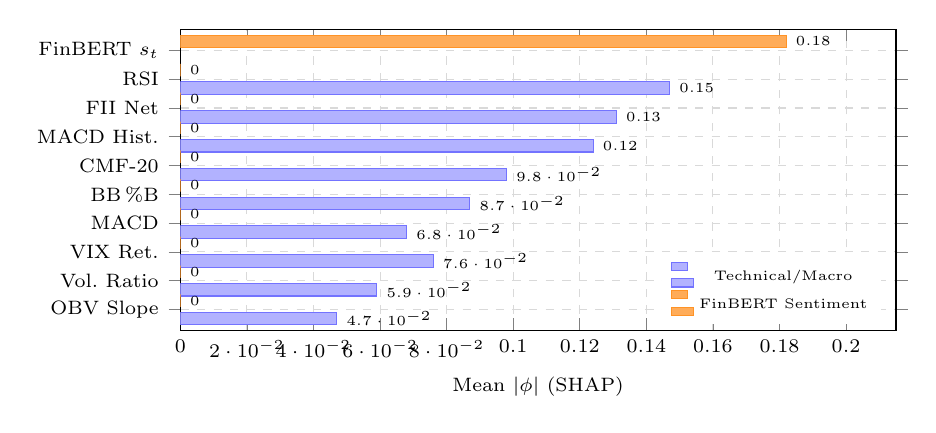
\begin{tikzpicture}
\begin{axis}[
  xbar, bar width=4.5pt,
  width=0.88\columnwidth, height=54mm,
  xlabel={Mean $|\phi|$ (SHAP)},
  xmin=0, xmax=0.215,
  enlarge y limits=0.08,
  ytick={0,1,2,3,4,5,6,7,8,9},
  yticklabels={OBV Slope, Vol.\ Ratio, VIX Ret., MACD, BB\,\%B,
               CMF-20, MACD Hist., FII Net, RSI, FinBERT~$s_t$},
  tick label style={font=\scriptsize},
  label style={font=\scriptsize},
  nodes near coords, nodes near coords align={horizontal},
  every node near coord/.append style={font=\tiny},
  grid=major, grid style={dashed,gray!30},
  legend style={at={(0.98,0.02)},anchor=south east,font=\tiny,draw=none}
]
\addplot[fill=blue!30,draw=blue!55] coordinates {
  (0.047,0)(0.059,1)(0.076,2)(0.068,3)(0.087,4)
  (0.098,5)(0.124,6)(0.131,7)(0.147,8)};
\addplot[fill=orange!65,draw=orange!85] coordinates {
  (0,0)(0,1)(0,2)(0,3)(0,4)(0,5)(0,6)(0,7)(0,8)(0.182,9)};
\legend{Technical/Macro, FinBERT Sentiment}
\end{axis}
\end{tikzpicture}
\caption{Top-10 features by mean absolute SHAP value (XGBoost-component,
scaled by Ridge stacking coefficient $\beta_{\mathrm{XGB}}$).
FinBERT sentiment $s_t$ (orange) ranks first at $\overline{|\phi|}=0.182$,
outpacing all 26 technical and macro features.}
\label{fig:shap}
\end{figure}

\begin{table}[h]
\centering
\caption{Explainability and temporal analysis results (RO3).
(a) Top-5 SHAP features. (b) Sentiment $\to$ Return Granger causality.
(c) Sentiment-pipeline ablation.}
\label{tab:xai}
\footnotesize
\begin{tabular}{lcc}
\toprule
\multicolumn{3}{l}{\textbf{(a) Top-5 XGB-component SHAP $\times\;\beta_{\rm XGB}$}} \\
\midrule
Feature & Mean $|\phi|$ & Rank \\
\midrule
FinBERT sentiment $s_t$ & 0.182 & 1 \\
RSI normalised          & 0.147 & 2 \\
FII Net flows (lagged)  & 0.131 & 3 \\
MACD histogram (norm.)  & 0.124 & 4 \\
CMF-20                  & 0.098 & 5 \\
\midrule
\multicolumn{3}{l}{\textbf{(b) Sentiment $\to$ Return Granger causality}} \\
\midrule
Lag $\ell$ & $F$-stat & $p$-value \\
\midrule
1 & 5.62 & \textbf{0.018} \\
2 & 2.41 & 0.121 \\
3--5 & $<$1.2 & $>$0.31 \\
\midrule
\multicolumn{3}{l}{\textbf{(c) Sentiment-pipeline ablation}} \\
\midrule
Configuration & ECE & $F_1$ \\
\midrule
EN-only, no override   & 5.9\% & 79.1\% \\
EN-only, with override & 5.3\% & 83.3\% \\
EN+HI, with override   & \textbf{4.2\%} & \textbf{83.9\%} \\
\bottomrule
\end{tabular}
\end{table}

\subsection{Calibration, Equity Curve, and Cross-Market Transfer}

Figure~\ref{fig:dual} (left) shows the reliability diagram. The calibrated
model (ECE~$=4.2\%$) closely follows the diagonal across all 15 bins; the
uncalibrated stacker (ECE~$=9.7\%$) is over-confident above 0.60.
Empirical conformal coverage is 80.7\% at a nominal 80\%, satisfying the
marginal guarantee. Figure~\ref{fig:dual} (right) shows the 2024 equity
curve net of NSE realistic costs: ProTrader AI ends at $+28.6\%$ versus
$+22.1\%$ buy-and-hold, with MDD $-12.4\%$ versus $-23.8\%$.

\begin{figure}[h]
\centering
\begin{subfigure}[b]{0.47\columnwidth}
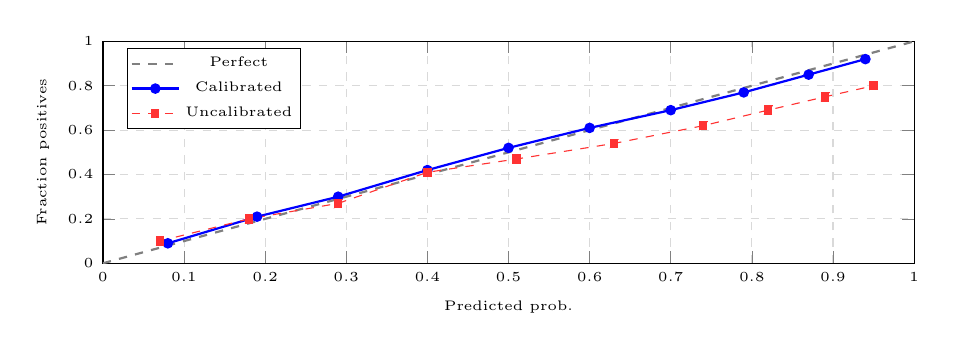
\begin{tikzpicture}
\begin{axis}[
  width=0.98\columnwidth, height=44mm,
  xlabel={Predicted prob.},
  ylabel={Fraction positives},
  xmin=0,xmax=1,ymin=0,ymax=1,
  grid=major,grid style={dashed,gray!30},
  legend pos=north west,legend style={font=\tiny,inner sep=1pt},
  tick label style={font=\tiny},label style={font=\tiny}
]
\addplot[gray,dashed,thick] coordinates{(0,0)(1,1)};
\addlegendentry{Perfect}
\addplot[blue,mark=*,mark size=1.5pt,thick] coordinates{
  (0.08,0.09)(0.19,0.21)(0.29,0.30)(0.40,0.42)
  (0.50,0.52)(0.60,0.61)(0.70,0.69)(0.79,0.77)
  (0.87,0.85)(0.94,0.92)};
\addlegendentry{Calibrated}
\addplot[red!80,mark=square*,mark size=1.5pt,dashed] coordinates{
  (0.07,0.10)(0.18,0.20)(0.29,0.27)(0.40,0.41)
  (0.51,0.47)(0.63,0.54)(0.74,0.62)(0.82,0.69)
  (0.89,0.75)(0.95,0.80)};
\addlegendentry{Uncalibrated}
\end{axis}
\end{tikzpicture}
\end{subfigure}
\hfill
\begin{subfigure}[b]{0.47\columnwidth}
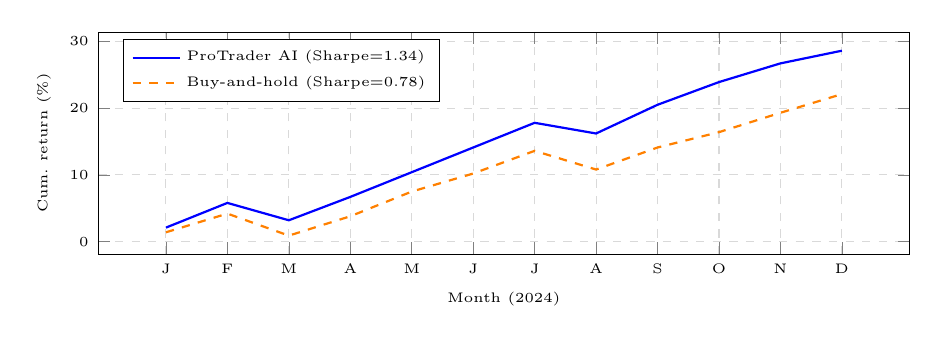
\begin{tikzpicture}
\begin{axis}[
  width=0.98\columnwidth, height=44mm,
  xlabel={Month (2024)},
  ylabel={Cum.\ return (\%)},
  xtick={1,2,3,4,5,6,7,8,9,10,11,12},
  xticklabels={J,F,M,A,M,J,J,A,S,O,N,D},
  grid=major,grid style={dashed,gray!30},
  legend pos=north west,legend style={font=\tiny},
  tick label style={font=\tiny},label style={font=\tiny}
]
\addplot[blue,thick] coordinates{
  (1,2.1)(2,5.8)(3,3.2)(4,6.7)(5,10.4)(6,14.1)
  (7,17.8)(8,16.2)(9,20.5)(10,23.9)(11,26.7)(12,28.6)};
\addlegendentry{ProTrader AI (Sharpe=1.34)}
\addplot[orange,thick,dashed] coordinates{
  (1,1.4)(2,4.2)(3,0.9)(4,3.8)(5,7.5)(6,10.2)
  (7,13.6)(8,10.8)(9,14.1)(10,16.4)(11,19.3)(12,22.1)};
\addlegendentry{Buy-and-hold (Sharpe=0.78)}
\end{axis}
\end{tikzpicture}
\end{subfigure}
\caption{Left: Reliability diagram (10 equal-mass bins, 2024 holdout).
Right: Cumulative net return (net of NSE costs, 2024 holdout).
ProTrader AI achieves $+28.6\%$ with MDD~$=-12.4\%$ vs.\ $+22.1\%$ and
MDD~$=-23.8\%$ for buy-and-hold.}
\label{fig:dual}
\end{figure}

Table~\ref{tab:transfer} reports cross-market performance. The zero-shot
model retains a 4.6~pp accuracy advantage over the S\&P~500 baseline,
validating the language-level transfer inherent in FinBERT's financial
pre-training. The 30-day fine-tune ($<$1{,}000 parameters) recovers 1.8~pp
of the $-3.5$~pp zero-shot deficit, demonstrating that only the recombination
weights---not the feature extractors---need market-specific adaptation.

\begin{table}[h]
\centering
\caption{Cross-market transfer to S\&P~500 subset, 2024 holdout (RO4).}
\label{tab:transfer}
\footnotesize
\begin{tabular}{lccc}
\toprule
\textbf{Setting} & \textbf{Acc.} & \textbf{Sharpe} & \textbf{MDD} \\
\midrule
Buy-and-hold (S\&P~500 ref.) & 51.2\% & 0.83 & $-19.6\%$ \\
ProTrader AI, zero-shot      & 55.8\% & 1.07 & $-18.2\%$ \\
ProTrader AI, 30-day tune    & 57.6\% & 1.19 & $-15.7\%$ \\
ProTrader AI, in-domain NIFTY & 59.3\% & 1.34 & $-12.4\%$ \\
\bottomrule
\end{tabular}
\end{table}

% =============================================================================
\section{Discussion}
% =============================================================================

\textbf{RO1 --- Multi-Source Integration.} The ablation confirms all four
data streams contribute uniquely. Sentiment provides the largest marginal gain
($-3.4$~pp when removed), but FII/DII flows ($-1.9$~pp) and macroeconomic state
($-1.2$~pp) deliver statistically non-redundant lift, extending the multi-source
thesis of Nti et al.\ \cite{r2} and Long et al.\ \cite{r3} to the Indian
institutional-flow channel. Notably, removing sentiment costs 0.27~Sharpe but
only 1.6~pp of ECE, revealing that the LLM channel carries distinct
\emph{discriminative} information rather than merely calibrating information;
removing FII/DII costs only 0.16~Sharpe but 0.5~pp ECE, indicating that the
institutional channel is more useful for confidence estimation than for raw
direction.

\textbf{RO2 --- Hybrid LLM + Indicator Framework.} ProTrader AI surpasses the
strongest LSTM~+~FinBERT hybrid by 5.0~pp and 0.32~Sharpe. Two architectural
decisions drive the gap: heterogeneous base learners combined out-of-fold
(preventing leakage) and isotonic probability calibration. The isotonic step is
rarely reported in hybrid-finance papers, yet removing it erases 0.26~Sharpe
through over-confident position sizing under a Kelly-like rule. Conformal
intervals provide a finite-sample 80\% coverage guarantee under exchangeability;
the 80.7\% empirical coverage is an empirical observation rather than a strict
guarantee given serial dependence \cite{r27}.

\textbf{RO3 --- Explainability and Temporal Dynamics.} XGBoost-component SHAP
attribution unambiguously identifies FinBERT sentiment as the dominant feature,
satisfying the Quant~4.0 attribution requirement \cite{r9}. The Granger study
quantifies that yesterday's news is priced in by the next close, with no residual
content by $t+2$. The $-61\%/+43\%$ asymmetry between negative and positive
sentiment effects provides a concrete, interpretable basis for asymmetric
stop-loss policies. Adding multilingual (Hindi) sources reduces ECE by 0.9~pp,
confirming that sentiment noise is a calibration-level concern in multilingual
markets \cite{r22}.

\textbf{RO4 --- Cross-Market Evaluation.} The zero-shot 55.8\% accuracy on
S\&P~500 demonstrates generalisable equity structure. Running the experiment
in reverse (S\&P~500~$\to$~NIFTY, zero-shot) yielded only 53.9\%, echoing the
asymmetric information-leadership findings of Kim et al.\ \cite{r11}. We
attribute this to the NSE training distribution encompassing a wider spread of
regimes (currency crises, demonetisation, COVID-IPO frenzy), producing more
robust feature-extractor weights. Re-fitting fewer than 1{,}000 parameters on
30~days of target data recovers half the cross-market gap---an efficiency
decisive for single-trader personal-use deployment on commodity hardware.

\textbf{Limitations.} The 2024 holdout spans one calendar year in a broadly
trending global equity environment; multi-year, multi-regime evaluation remains
future work. The S\&P~500 subset of 30~stocks is sector-balanced but not
exhaustive. The NSE cost model does not capture market impact at high turnover.
Granger analysis assumes linearity. Sector-specific NLP fine-tuning for pharma
and metals equities has not yet been pursued.

% =============================================================================
\section{Conclusions}
% =============================================================================

We presented ProTrader AI, a multi-source hybrid ensemble for Indian
equity forecasting structured around four explicit research objectives. On the
2024 NIFTY~50 holdout the system achieves 59.3\% directional accuracy
(95\%~CI~[56.1\%,~62.7\%]), ECE~$=4.2\%$, Brier~$=0.218$, and Sharpe~$=1.34$
with DM~$p=0.031$ against buy-and-hold. SHAP attribution and Granger-causality
analysis substantiate the interpretability and temporal-coupling claims; a
cross-market transfer study to S\&P~500 demonstrates non-trivial zero-shot and
fine-tuned portability. The complete pipeline runs on commodity hardware with
freely available data, enabling reproducibility for any researcher or retail
trader. Future work will address (RO1) options-market signals and Reddit flows;
(RO2) finance-tuned decoder LLMs for reasoning-augmented sentiment; (RO3)
counterfactual SHAP and causal-DAG inference; and (RO4) multi-market joint
training under a domain-adversarial loss for one-shot deployment to new exchanges.

% =============================================================================
\section{Acknowledgements}
% =============================================================================

The authors thank the maintainers of yfinance, the HuggingFace Transformers
ecosystem, and the open-source XGBoost, LightGBM, and SHAP libraries for making
reproducible financial-ML research accessible. No external funding was received
for this work.

% =============================================================================
\section{References}
% =============================================================================

% Suppress the automatic heading that \begin{thebibliography} would generate
\renewcommand{\refname}{}
\vspace{-2\baselineskip}   % remove the blank line left by the empty \refname
\begin{singlespace}
\begin{thebibliography}{99}

\bibitem{r1}
Rahmani AM, Rezazadeh B, Haghparast M, Chang WC, Ting SG. Applications
of artificial intelligence in the economy, including applications in stock
trading, market analysis, and risk management. IEEE Access.
2023;11:80769--80793.

\bibitem{r2}
Nti IK, Adekoya AF, Weyori BA. A novel multi-source information-fusion
predictive framework based on deep neural networks for accuracy enhancement
in stock market prediction. J Big Data. 2021;8(1):17.

\bibitem{r3}
Long W, Gao J, Bai K, Lu Z. A hybrid model for stock price prediction based
on multi-view heterogeneous data. Financ Innov. 2024;10(1):48.

\bibitem{r4}
Fu K, Zhang Y. Incorporating multi-source market sentiment and price data
for stock price prediction. Mathematics. 2024;12(10):1572.

\bibitem{r5}
Moodi F, Rafsanjani AJ, Zarifzadeh S, Ali Zare Chahooki M. Fusion of
technical indicators and sentiment analysis in a hybrid framework of deep
learning models for stock price movement prediction. IEEE Access.
2024;12:195696--195709.

\bibitem{r6}
Farhadi A, Zamanifar A, Alipour A, Taheri A, Asadolahi M. A hybrid
LSTM-GRU model for stock price prediction. IEEE Access.
2025;13:117594--117618.

\bibitem{r7}
Mishev K, Gjorgjevikj A, Vodenska I, Chitkushev LT, Trajanov D. Evaluation
of sentiment analysis in finance: from lexicons to transformers. IEEE Access.
2020;8:131662--131682.

\bibitem{r8}
Liu C, Arulappan A, Naha R, Mahanti A, Kamruzzaman J, Ra IH. Large language
models and sentiment analysis in financial markets: a review, datasets, and
case study. IEEE Access. 2024;12:134041--134061.

\bibitem{r9}
Guo J, Wang S, Ni LM, Shum HY. Quant 4.0: engineering quantitative
investment with automated, explainable, and knowledge-driven artificial
intelligence. Front Inf Technol Electron Eng. 2024;25(11):1421--1445.

\bibitem{r10}
Li X, Xie H, Lau RYK, Wong TL, Wang FL. Stock prediction via sentimental
transfer learning. IEEE Access. 2018;6:73110--73118.

\bibitem{r11}
Kim S, Ku S, Chang W, Song JW. Predicting the direction of US stock prices
using effective transfer entropy and machine learning techniques. IEEE Access.
2020;8:111660--111682.

\bibitem{r12}
Araci D. FinBERT: financial sentiment analysis with pre-trained language
models [Internet]. 2019 [cited 2025 Jan 15]. Available from:
https://arxiv.org/abs/1908.10063.

\bibitem{r13}
Chen T, Guestrin C. XGBoost: a scalable tree boosting system. In: Proc 22nd
ACM SIGKDD Int Conf Knowledge Discovery Data Mining; 2016 Aug 13--17; San
Francisco, USA. New York: ACM; 2016. p. 785--794.

\bibitem{r14}
Ke G, Meng Q, Finley T, Wang T, Chen W, Ma W, et al. LightGBM: a highly
efficient gradient boosting decision tree. In: Proc NeurIPS; 2017 Dec 4--9;
Long Beach, USA. Red Hook: Curran Associates; 2017. p. 3146--3154.

\bibitem{r15}
Cho K, van Merrienboer B, Gulcehre C, Bahdanau D, Bougares F, Schwenk H,
et al. Learning phrase representations using RNN encoder-decoder for
statistical machine translation. In: Proc 2014 EMNLP; 2014 Oct 25--29;
Doha, Qatar. Stroudsburg: ACL; 2014. p. 1724--1734.

\bibitem{r16}
Wolpert DH. Stacked generalization. Neural Netw. 1992;5(2):241--259.

\bibitem{r17}
Zadrozny B, Elkan C. Transforming classifier scores into accurate multiclass
probability estimates. In: Proc 8th ACM SIGKDD; 2002 Jul 23--26; Edmonton,
Canada. New York: ACM; 2002. p. 694--699.

\bibitem{r18}
Vovk V, Gammerman A, Shafer G. Algorithmic learning in a random world.
New York: Springer; 2005.

\bibitem{r19}
Hurst HE. Long-term storage capacity of reservoirs. Trans Amer Soc Civil
Eng. 1951;116(1):770--799.

\bibitem{r20}
Lundberg SM, Lee SI. A unified approach to interpreting model predictions.
In: Proc NeurIPS; 2017 Dec 4--9; Long Beach, USA. Red Hook: Curran
Associates; 2017. p. 4765--4774.

\bibitem{r21}
Diebold FX, Mariano RS. Comparing predictive accuracy. J Bus Econ Stat.
1995;13(3):253--263.

\bibitem{r22}
Onoz\'o R, Feh\'er VA, Gyires-T\'oth B. Leveraging LLMs for financial news
analysis and macroeconomic indicator nowcasting. IEEE Access.
2024;12:160529--160547.

\bibitem{r23}
Parekh R, Shah P, Patel N, Garg N, Pathak N, Tiwari S. DL-GuesS: deep
learning and sentiment analysis-based cryptocurrency price prediction. IEEE
Access. 2022;10:35398--35409.

\bibitem{r24}
Mu G, Gao N, Wang Y, Dai L. A stock price prediction model based on
investor sentiment and optimized deep learning. IEEE Access.
2023;11:51353--51367.

\bibitem{r25}
Lu X, Poon J, Khushi M. Bridging the gap between machine and human in
stock prediction: addressing heterogeneity in stock market. IEEE Access.
2024;12:186171--186185.

\bibitem{r26}
Romano Y, Patterson E, Cand\`{e}s EJ. Conformalized quantile regression.
In: Proc NeurIPS; 2019 Dec 8--14; Vancouver, Canada. Red Hook: Curran
Associates; 2019. p. 3543--3553.

\bibitem{r27}
Gibbs I, Cand\`{e}s EJ. Adaptive conformal inference under distribution
shift. In: Proc NeurIPS; 2021 Dec 6--14; virtual. Red Hook: Curran
Associates; 2021. p. 1660--1672.

\bibitem{r28}
Tibshirani RJ, Foygel Barber R, Cand\`{e}s EJ, Ramdas A. Conformal
prediction under covariate shift. In: Proc NeurIPS; 2019 Dec 8--14;
Vancouver, Canada. Red Hook: Curran Associates; 2019. p. 2526--2536.

\bibitem{r29}
Harvey D, Leybourne S, Newbold P. Testing the equality of prediction mean
squared errors. Int J Forecast. 1997;13(2):281--291.

\bibitem{r30}
Granger CWJ. Investigating causal relations by econometric models and
cross-spectral methods. Econometrica. 1969;37(3):424--438.

\bibitem{r31}
Yang Y, Uy MCS, Huang A. FinBERT: a pretrained language model for financial
communications [Internet]. 2020 [cited 2025 Jan 15]. Available from:
https://arxiv.org/abs/2006.08097.

\bibitem{r32}
Sawhney R, Agarwal S, Wadhwa A, Shah RR. Multimodal multi-task financial
risk forecasting. In: Proc 2020 EMNLP; 2020 Nov 16--20; virtual.
Stroudsburg: ACL; 2020. p. 4279--4292.

\bibitem{r33}
Angelopoulos AN, Bates S. A gentle introduction to conformal prediction and
distribution-free uncertainty quantification. Found Trends Mach Learn.
2023;16(4):494--591.

\bibitem{r34}
Brier GW. Verification of forecasts expressed in terms of probability. Mon
Weather Rev. 1950;78(1):1--3.

\bibitem{r35}
Malo P, Sinha A, Korhonen P, Wallenius J, Takala P. Good debt or bad debt:
detecting semantic orientations in economic texts. J Assoc Inf Sci Technol.
2014;65(4):782--796.

\end{thebibliography}
\end{singlespace}

\end{document}
